\chapter{Lo scenario applicativo}
\label{scenario}
In questo capitolo si illustra brevemente il concetto di vulnerabilità e l'equazione concettuale che esprime il legame tra l'impatto di un disastro ed essa. Viene quindi spiegato un framework ciclico per il disaster-management e si sfatano i luoghi comuni legati al contesto di questa tesi. Contesto che viene infine definito nell'ultimo paragrafo.


\section{La vulnerabilità}
\label{vuln}

La parola vulnerabilità \cite{NOTE} deriva dal latino "\textit{vulnerare}" che significa ferire. Principalmente si riferisce all'esporre persone, beni e arrività a potenziali danni e/o perdite. \\
La vulnerabilità è un concetto astratto, ma comunque reale, difficilmente misurabile.  La sua esistenza si percepisce successivamente ad un evento, verificando l'impatto del disastro stesso. Dunque è una proprietà latente o intrinseca.\\
Uno dei grandi risultati di studi disastri nella seconda metà del XX secolo è stato quello di stabilire che la vulnerabilità è la componente principale del rischio ( Hewitt 1983). In formulazioni più estreme, il pericolo (l'altro principale componente) è considerato come la probabilità che accada un fenomeno dannoso e la vulnerabilità la propensione a subire danni. E' stata quindi formulata un'equazione concettuale che lega questi concetti, ovvero:
\begin{equation}
\label{eq}
Pericolo * (Vulnerabilit\grave{a} *Esposizione ) = Rischio \rightarrow Impatto
\end{equation}
\newpage
Per \textbf{Pericolo} si intende la probabilità che un certo fenomeno colpisca una certa area mentre per \textbf{Esposizione} si intende il lasso di tempo nel quale, una persona, o una risorsa è minacciata da un particolare rischio. 
Dato il ruolo di \textit{Esposizione} , è importante notare che la vulnerabilità non è un concetto "tutto o niente ". \\
Molti studi di rischio sono basati sulla propensione alle perdite totali. Questo, naturalmente, presuppone una totale incapacità di resistere all'impatto del disastro. E' necessario quindi introdurre un altro concetto: la \textbf{Resilienza}.
La resilienza deriva dal comportamento fisico dei materiali, e si riferisce alla capacità di una sostanza ( o in questo caso della società ) di assorbire e resistere al trauma di un disastro. È, ovviamente, l'inverso della vulnerabilità; possiamo quindi raffinare l'equazione precedente: 
\begin{center}
$Pericolo * (Vulnerabilit\grave{a} * Esposizione ) / Resilienza = Rischio \rightarrow Impatto$
\end{center}
Quindi, la \textbf{Vulnerabilità} può essere anche parziale. Se è quantificabile può essere espressa come un indice o una percentuale relativa alla perdita totale. Se può essere stimata si possono usare varie metriche, come la gravità dei danni rispetto alla letalità oppure i gradi di perdita dell'integrità strutturale di un edificio rispetto al suo collasso totale.\\
La possibilità di disaggregare la vulnerabilità in varie componenti indica che questa può assumere diverse forme, tuttavia queste non sono indipendenti le une dalle altre. Una possibile interpretazione della vulnerabilità è che\textbf{ può essere definita rispetto alle circostanze che la generano}. Il seguente modello la scompone in funzione del contesto ( Alexander 1997 Özerdem e Jacoby 2006):
\begin{itemize}
\item \textbf{Vulnerabilità totale:} la vita è generalmente precaria perché poco o nulla è stato fatto per ridurre le fonti e i pontenziali rischi di impatti. Questa condizione tende a manifestarsi sopratutto nelle società più povere ed emarginate che non dispongono delle risorse per proteggersi.
\item \textbf{Economici:} le persone non hanno un'adeguata occupazione, quindi la vulnerabilità si riferisce alla precareità delle loro attività produttive e alle fonti di reddito.
\item \textbf{Tecnologia:} causata dalla pericolosità della tecnologia o dal modo in cui viene usata.
\item \textbf{Delinquenti:} causata dalla corruzione, negligenza o attività criminali che mettono in pericolo le persone e i beni.
\item\textbf{ Appena generato:} causato dal cambiamento delle circostanze , per esempio a causa di rischi emergenti .
\end{itemize}
 Data l'etereogenità delle moderne società , tali categorie non sono mutue esclusive. \\
 Se accettiamo che la vulnerabilità può assumere diverse forme, allora dobbiamo tener conto delle possibili interazioni tra le varie componenti. Possiamo definire:
 \begin{itemize}
 \item \textbf{Vulnerabilità primaria:} il prodotto diretto tra causa ed effetto. Ad esempio, se un terremoto squote una casa, la scarsa qualità delle murature potrebbe causare il crollo totale della costruzione.
 \item \textbf{Vulnerabilità secondaria:} è il risultato dell'interazione tra le cause o il verificarsi di coincidenze. Ad esempio, un edificio può resistere alle scosse di un terremoto ma non all'inondazione causata dal collasso di una diga a monte (Disastro del Vajont).
 \item \textbf{Vulnerabilità complessa:} si presenta quando le complicate interazioni tra le componenti aumentano complessivamente la vulnerabilità. Gli effetti economici ramificati di un forte terremoto, in una città metropolitana, ne sono un chiaro esempio.
 \end{itemize}
 La vulnerabilità non è statica, se in questo momento qualcuno è \textit{"vulnerabile"}, questo non implica che lo sarà futuro; analogamente vale il viceversa, le persone potrebbero diventare vulnerabili a causa di forze o processi come l'invecchiamento o la malattia che sono eventi indipendenti dai disastri. Quindi \textbf{l'analisi della vulnerabilità può essere vista come un'istantanea di un processo dinamico} e come tale ha una validità temporale limitata. \\
La vulnerabilità può essere misurata o stimata direttamente come il pontenziale danno o perdita oppure, in modo indiretto misurando la non resilienza. Queste misure richiedono però di ipotizzare il potenziale impatto di un probabile evento non avvenuto, di consenguenza la presenza di errori è inevitabile. \\
In conclusione le misure prese per ridurre la vulnerabilità devono essere sostenibili; inoltre devono essere locali, supportate dalla comunità, ben integrate nella legislazione e pianificate al fine di rendere la vita degli abitanti, della zona in questione, più \textit{"resistente"}. \newpage



\section{Le fasi di emergency management}
\label{fasi}
Per aumentare la "resilienza" (vedi \ref{vuln}) della comunità è necessario prepararsi in tempi di pace, saper gestire i disastri e cercare di prevenirli quando possibile. Tutte queste attività prendono il nome di \textbf{Emergency management}.	\\
Il termine "emergency management" è usato per indicare tutte quelle attività, condotte da agenzie private o pubbliche, che hanno lo scopo di fornire supporto e assistenza ai territori colpiti da disastri ambientali e/o umani. \\
La gestione di tali cataclismi, può essere divisa in quattro fasi, come illustrato in Figura 1.1 :

\begin{figure}[H]
	\centering
	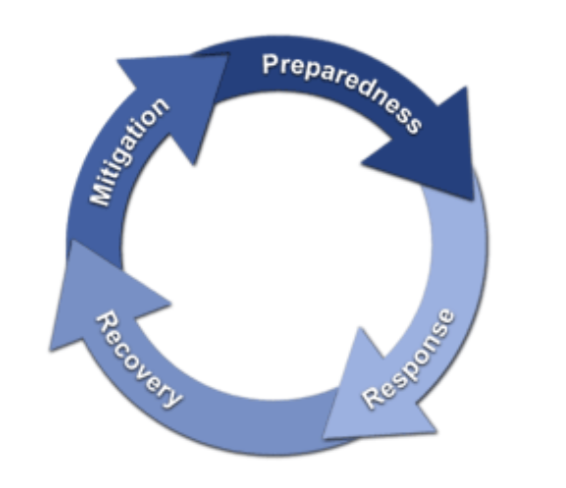
\includegraphics[scale=0.8]{ScenarioApplicativo/disaster_phase.png}
	\caption{Ciclo di fasi per il disaster-management}
	\label{fig:contesto_cycle}
\end{figure}
 \newpage
 Le definizioni di queste fasi sono svariate e variano a seconda dell'agenzia che le fornisce; a grandi linee possono essere così descritte \cite{FASI_MANAGEMENT}:
 \begin{itemize}
 \item \textbf{Mitigation:} Include tutte quelle attività svolte per ridurre le perdite di vite e proprietà a causa di un disastro naturale e/o umano: \textit{"un'azione continua che riduce o elimina il rischio a lungo termine per le persone e le proprietà da pericoli naturali e dai loro effetti"}. L'attuazione di strategie di Mitigation è una parte della fase di Recovery se applicata dopo il verificarsi di un disastro.\\
Le misure di Mitigation possono essere:
\begin{itemize}
\item\textbf{Strutturali}, forniscono soluzioni tecnologiche, come l'ampliamento degli argini di un fiume.
\item\textbf{Non strutturali}, forniscono soluzione legislative, come il divieto di costruzione su terreni paludosi.
\end{itemize}
\item \textbf{Preparednes:} Ha lo scopo di preparare al meglio la comunità attraverso attività formative.\\
Questa fase è un continuo ciclo di pianificazione, organizzazione, prove e valutazioni; in questo modo l'emergency manager sarà in grado di fornire la miglior soluzione.\\
Nella fase di preparednes si sviluppano piani d'azione per gestire e contrastare i rischi e si costruiscono le risorse necessarie per attuare tali piani. Alcune misure comuni sono: 
\begin{itemize}
\item Comunicazione dei piani con terminologia e metodi comprensibili.
\item Corretta manutenzione dei servizi d'emergenza.
\item Sviluppo ed esercizio di metodi di avviso emergenza per la popolazione.
\item Creazione di rifugi e piani di evacuazione
\end{itemize}
\newpage
\item \textbf{Response:} Include la mobilitazione dei servizi di emeregenza necessari e primi interventi nell'area colpita; è probabile che includano una prima ondata di servizi base come pompieri, polizia e ambulanze. \\
In particolare in questa fase si attuano i piani precedentemente ideati nella fase di preparednes e le attività dovrebbero includere:
\begin{itemize}
\item Ricerca e soccorso.
\item Distribuire viveri e medicinali
\item Valutazione dei danni
\item Riparo per le vittime
\item Estinzione di eventuali incendi
\end{itemize}
\item \textbf{Recovery:} Include tutte quelle attività che hanno l'obiettivo di riportare le persone alla loro "normalità". Riparazione, sostituzione e ricostruzione sono esempi tipici.\\
Lo scopo della fase di Recovery è appunto ripristinare l'area colpita allo stato precedente la catastrofe, tuttavia le azioni devono essere eseguite soltanto quando i bisogni della comunità sono stati soddisfatti e la fase di Response è quindi terminata; a quel punto si possono avviare le attività di ripristino con lo sforzo di "ricostruire indietro meglio", cioè provando a ridurre i rischi, precedenti al disastro, presenti nella comunità e nelle infrastrutture.\\
La fase di Recovery può essere divisa in due periodi. La fase a breve termine, in genere, dura da sei mesi almeno ad un anno e prevede la fornitura di servizi immediati alle imprese. La fase a lungo termine, che può durare anche decenni, richiede una pianificazione strategica efficente per affrontare gli impatti più gravi e permanenti di un disastro. \\
Le comunità devono accedere e distribuire una vasta gamma di risorse pubbliche e private per consentire la ripresa economica a lungo termine.
\end{itemize}
Un utilizzo ottimale di questo framework è in grado di fornire alla comunità le risorse necessarie affinché un disastro possa essere affrontato in maniera efficace, o meglio, si possono ridurre tutte quelle morti causate dalla negligenza di "involucri organici", privi di qualsiasi etica e morale erroneamente chiamati professionisti.
\newpage


\section{I luoghi comuni sui disastri}
\label{comuni}
Se ci venisse chiesto di immaginare lo scenario immediato ad un disastro ambientale o umano, nella maggior parte dei casi, potremmo scrivere una buona trama per un film apocalittico. Questo succede a causa di alcuni luoghi comuni diffusi nella nostra società \cite{COMMON}, ciò che ci sembra ovvio infatti potrebbe essere soltanto un mito inculcato nella nostra mente:
\begin{enumerate}
\item\textbf{ I disastri sono eventi rari}, sono una parte normale della vita quotidiana e in molti casi sono eventi ripetitivi.
\item\textbf{ I disastri naturali sono inevitabilmente il risultato della furia di madre natura}, le cause di questi eventi sono sì naturali, infatti non possiamo fare niente per eliminare i terremoti, le inondazioni o le tempeste tropicali. Tuttavia, il disastro è quasi sempre causato dalle persone e dalle comunità stesse che si mettendo in condizioni di rischio e non vi è nulla di molto naturale o inevitabile in tutto questo. 
\item\textbf{ I disastri provocano una grande quantità di caos e non possono essere gestiti in modo sistematico}, ci sono ottimi modelli teorici su come disastri funzionano e come gestirli. Dopo più di 75 anni di ricerca nel campo, gli elementi generali del disastro sono ben noti, e tendono a ripetersi da un disastro all'altro.
\item\textbf{ I disastri uccidono le persone indipendetemente dal loro status sociale o economico }, le persone povere ed emarginate sono molto più a rischio di morte di quelle ricche e benestanti.
\item\textbf{ I terremoti sono comunemente responsabili di bilanci molto elevati di morte.}, gli edifici che crollano sono i veri responsabili. Come già detto non è possibile fermare i terremoti, è possibile però costruire edifici antisismici e organizzare attività umane in modo tale da minimizzare il rischio di morte.
\item\textbf{Quando avviene il disastro il panico è la reazione più comune}, la maggior parte delle persone mantiene un comportamento razionale. Il panico non è comunque da escludere.
\item\textbf{Un gran numero di persone fuggirà dall'area colpita}, di solito c'è un "reazione di convergenza" e la zona si riempie di persone. Alcuni dei sopravvissuti se ne andranno, altri saranno evecuati ma durerà comunque poco.
\item\textbf{Dopo il disastro i sopravvissuti tendono ad essere storditi e apatici}, i sopravvissuti tendono a mettersi al lavoro per "ripulire". L'attivismo è molto più comune della rassegnazione (questa è la cosiddetta "comunità terapeutica"). Nel peggiore dei casi solo il 15-30 per cento delle vittime mostrano reazioni passive.
\item\textbf{Le persone tendono a prendere decisioni sbagliati a meno che non siano guidati dalle autorità}, le persone prendono decisioni sulla base delle informazioni che sono in grado di ottenere e di interpretare. All'interno di questa "bussola", la maggior parte del processo decisionale può essere giudicato razionale.
\item\textbf{ I disastri di solito danno luogo a diffuse manifestazioni spontanee di comportamento antisociale}, in generale i comportamenti sono caratterizzati da una grande solidarietà sociale, generosità e sacrificio di sé stessi.
\item\textbf{Il saccheggio è un fenomeno comune}, il fenomeno dei saccheggi è raro e di portata limitata. Si verifica soprattutto quando ci sono presupposti forti, come quando una comunità è già profondamente divisa.
\item\textbf{Le persone ricorrono alla violenza per proteggere i propri interessi}, La \textit{'comunità terapeutica'} è comune, infatti le persone hanno una maggiore tendenza ad aiutarsi a vicenda in situazioni d'emergenza che in tempi normali.
\item\textbf{La legge marziale deve essere imposta dopo il disastro al fine di evitare che la società si rompa del tutto}, L'imposizione della legge marziale dopo il disastro è estremamente raro, ad ogni modo il suo utilizzo implica che i normali meccanismi di governo non sono mai stati efficaci.
\item\textbf{I cadeveri non seppelliti costituiscono un pericolo per la salute}, Nemmeno la decomposizione costituisce un significativo rischio per la salute. Seppelire in modo avventato demoralizza i sopravvissuti e sconvolge le modalità di certificazione di morte, i riti funebri, e, ove necessario, l'autopsia.
\item\textbf{Le epidemie sono risultati quasi inevitabili delle distruzioni e delle scarse condizioni salutari causate dalla maggior parte dei disastri }, in generale, il livello di sorveglianza epidemiologica e l'assistenza sanitaria nella zona del disastro è sufficiente per fermare ogni possibile epidemia. Tuttavia, il tasso di diagnosi di malattie può aumentare con una migliore assistenza sanitaria, sopratutto in aree molto povere.
 \item\textbf{Una grande quantità e assortimento di medicinali dovrebbe essere inviato},  gli ospedali da campo sono solitamente installati troppo tardi per curare i feriti, finiscono per fornire assistenza generale e continuità delle cure. Poiché il trasporto e il funzionamento di questi tende ad essere costoso e logisticamente impegnativo, in alcuni casi può essere più efficiente per tentare di ripristinare o aumentare ospedali esistenti nel settore, anche se sono significativamente danneggiati.
 \item\textbf{A seguito di un disastro la vaccinazione di massa è un ottima strategia per fermare la diffusione di malattie},  considerando che la vaccinazione mirata di gruppi specifici (ad esempio, bambini, medici e infermieri) può essere una strategia efficace, la vaccinazione di massa indiscriminata è invece uno spreco.
 \item\textbf{I cadaveri, i sopravvissuti, strade, macerie e altre cose devono essere irrorati con un disinfettante per fermare la diffusione della malattia}, questa misura comune e popolare spreca grandi quantità di disinfettante e non fa assolutamente nulla per la salute pubblica.
 \item\textbf{Di solito c'è una carenza di risorse quando si verifica un disastro e questo impedisce di gestirlo in modo efficace}, le carenze se si verificano, sono quasi sempre molto provvisorie. In realtà ci sono più problemi nella buona distribuzione e utilizzo in modo efficiente rispetto all'acquisto vero e proprio.
\item\textbf{Qualsiasi tipo di aiuto è utile dopo il disastro purché sia fornito abbastanza rapidamente}, iniziative avventate e frettolose tendono a creare il caos. Inoltre saranno necessari solo alcuni tipi di assistenza tecnica, beni e servizi; infatti non tutte le risorse utili preesistenti il disastro saranno distrutti. La donazione di materiali inutilizzabili o manodopera consuma risorse di organizzazione e di alloggio che potrebbero più proficuamente essere utilizzate per ridurre il bilancio del disastro.
\item\textbf{Al fine di gestire al meglio un disastro è necessario accettare qualsiasi aiuto venga offerto}, è molto meglio limitarsi ad accettare donazioni di beni e servizi che sono effettivamente necessari nella zona del disastro.
\item\textbf{C'è un fenomeno noto come "terremoto tempo"}, la credenza popolare che i terremoti si verifichino quando vi è un clima afoso non ha alcuna base di fatto. Numerosi studi scientifici hanno cercato di individuare le condizioni atmosferiche precursorie ad un terremoto, ma l'unica osservazione riguarda il rilascio di alogeni nell'atmosfera.
\item\textbf{Gli animali sono in grado di percepire il terremoto prima che accada}, in realtà gli animali si comportano in modo insolito prima di un terremoto, tuttavia non è un modo affidabile di sapere se tale fenomeno sta per accadere.
\item\textbf{Siamo ben organizzati ad affrontare una pandemia o un attacco nucleare}, nella maggior parte dei paesi, compresi quelli più ricchi e più grandi, la fase di Preparedness è quella più trascurata e carente.
\item\textbf{In caso di un attacco terroristico biologico siamo in grado di confinare l'epidemia in modo efficace}, le scorte di anticorpi e vaccini sono insufficienti così come, i reparti di isolamento, le unità di risposta sul campo, le unità di decontaminazione, e la formazione per i soccorritori e medici. Inoltre potrebbe anche essere difficile da individuazione tempestivamente l'agente patogeno o la tossina in questione.
\item\textbf{Il panico e comportamenti irrazionali sono inevitabili conseguenze di un attacco terroristico nucleare}, in disastri di ogni genere maggior parte delle persone si sforzano di comportarsi razionalmente e prendere decisioni razionali . Questo è antitetica al panico. Tuttavia, se le persone non hanno informazioni adeguate, il loro processo decisionale può sottrarsi all'analisi razionale.
\item\textbf{I soccorritori non si presenterebbero in caso di disastro, poiché impegnati a proteggere la propria famiglia}, non è comune l'assenteismo di massa tra i soccorritori. In generale, le persone tendono ad avere un maggiore senso del dovere.
\item\textbf{I disastri accadono sempre a qualcun altro}, la sindrome dell' invulnerabilità personale, induce erroneamente le persone a ritenere che siano in qualche modo immune da disastri. Non è così.
\item\textbf{Scorte di sangue ed emoderivati devono essere inviati nei paesi stranieri colpiti}, ci sono ragioni patologiche e logistiche per le quali è meglio acquisire sangue ed emoderivati da donatori dello stesso paese colpito.
\item\textbf{Quando si verificano disastri gli adulti normodotati dovrebbero volontariamente aiutare }, l'era del volontariato spontaneo è finita. I volontari non organizzati portano più problemi di quanti ne risolvino. La risposta è quella di creare, in tempi di pace, associazioni di volontari addestrati ed equipaggiati, che possano essere integrati nel sistema di protezione civile per legge o secondo regole ben definite che definiscono i propri compiti e responsabilità.
\item\textbf{Vittime della carestia di solito muoiono di fame}, il più delle volte muoiono a causa di effetti colleterali della carestia, come la malnutrizione, diarrea, il tifo o il colera.
\item\textbf{Solo la preparazione porta ad agire}, produrre i mezzi per ridurre il rischio di catastrofi (un sistema di allarme, una mappa di pericolosità, un avanzamento delle tecniche costruttive antisismiche, di un regolamento edilizio aggiornato, ecc), non implica che verranno utilizzati; infatti la mancanza di leadership, cattive intenzioni, paralisi politica e la mancanza di fondi sono alcune possibili ragioni per cui questi mezzi potrebbero non essere utilizzati.

\end{enumerate}
\newpage

\section{Il contesto d'uso}
\label{contesto}
Questa tesi si colloca nel contesto di un lavoro di ricerca portato avanti da diversi anni da alcuni ricercatori del dipartimento DISIM.\\
Il team di ricerca ha condotto studi approfonditi sull'utilizzo dei sistemi ICT a supporto del disaster-management e prototipato diversi sistemi in questo ambito, basandosi anche sull'esperienza diretta del terremoto che colpì L'Aquila nel 2009.\\
Una delle attività più recenti di questo contesto è relativa ad un sistema che nella prima fase di \textit{Response} (vedi \ref{fasi}), possa supportare i  soccorritori (e le vittime) nell'esplorazione del territtorio colpito da un disastro. \\
\begin{figure}[H]
	\centering
	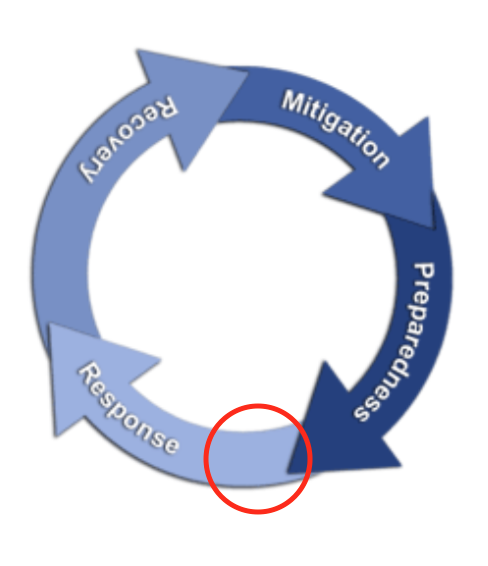
\includegraphics[scale=0.8]{ScenarioApplicativo/contesto.png}
	\caption{Contesto d'uso del sistema all'interno del disaster-management cycle}
	\label{fig:contesto}
\end{figure}
La soluzione proposta dal team integra l'attività di pianificazione e la \textbf{conoscenza dinamica del territorio} all'interno di un sistema multiagent-oriented per poter guidare le attività dei soccorritori (per maggiori dettagli si consiglia la visione del documento: "Disaster Response: a Multi-Agent based Approach" \cite{RESPONSE}).\\
La conoscenza dinamica è una caratteristica cruciale per sistemi di questo dominio applicativo; infatti un disastro naturale come il terremoto, può cambiare profondamente la morfologia del territorio rendendo gli strumenti OGB (Only-GPS-Based) non adatti a fornire soluzioni efficaci. I soccorritori, sopratutto quelli non locali, possono avere molte difficoltà nel raggiungere le vittime.
\newpage
L'acquisizione dinamica d'informazioni, benché utile alla conoscenza morfologica del territorio, è rilevante soprattutto per il coordinamento generale dei soccorritori, i cui piani d'azione non possono basarsi soltanto sulle considerazioni fatte nella fase di \textit{Preparedness} (vedi \ref{fasi}).\\
 Le strategie adottate dipendono dall'analisi preventiva della vulnerabilità (vedi \ref{vuln}), che a sua volta, dipende dalla stima del potenziale impatto di un disastro.\\
 E' chiaro che, in questo contesto, la disponibilità di dati dinamici permetterebbe ai soccorritori di rielabolare tali strategie a seconda del reale impatto. 
L'utilizzo di un MAS (multy agent system) presenta altri vantaggi, tra questi i più significativi sono: la possibilità di distribuire il carico computazionale e l'aumento della robustezza globale del sistema per mezzo di funzioni avanzate come l'automonitoraggio e l'autodiagnosi.\\
L'acquisizione dinamica delle informazioni può avvenire tramite droidi, sensori, robot e operatori umani incluse le stesse vittime; quest'ultime infatti utilizzando l'applicazione sviluppata in questa tesi, possono comunicare informazioni molto semplici e dirette tipiche del contesto (esempio "immediato aiuto qui") ai soccorritori. L'applicazione mobile risulterebbe uno strumento valido ed utilizzato dalle vittime: in accordo con i miti sfatati da D. Alexander (vedi in particolare i miti 6-8-10 in \ref{comuni}), è allora più che ragionevole utilizzare l'enorme quantità di informazioni che possono provenire dai sopravvissuti. Si noti che nelle prime 12-24 ore dopo il disastro le persone tendono, con o senza il sistema, a trasmettersi brevi messaggi significativi come "sono vivo", " la strada è bloccata qui", "c'è urgente bisogno di aiuto" ect permettendo la realizzazione di un sistema sia semplice da utilizzare anche da persone con poca familiarità con la tecnologia e nelle condizioni critiche caratterizanti del contesto, sia in grado di limitare, per quanto possibile, il numero di informazioni trasmesse.\\
 In conclusione l'implementazione di tale sistema contribuirebbe ad aumentare la \textit{Resilienza} della comunità (vedi \ref{vuln}), ovvero \textit{l'impatto} (vedi l'equazione \ref{eq}) e quindi le vittime. 